% Latex template: mahmoud.s.fahmy@students.kasralainy.edu.eg
% For more details: https://www.sharelatex.com/learn/Beamer

\documentclass{beamer}					% Document class

\usepackage[english]{babel}				% Set language
\usepackage[utf8x]{inputenc}			% Set encoding

% \usetheme{metropolis} % Preferred beamer theme

\usepackage{graphicx} % Load graphics
\usepackage{booktabs} % Nice tables
\usepackage{dcolumn} % Booktabs column spacing
\usepackage{threeparttable} % Align column caption, table, and notes
\usepackage{adjustbox} % Shrink stuff
\usepackage{showframe} % Useful for debugging

% Fancy fit image command with optional caption
\makeatletter
\newcommand{\fitimage}[2][\@nil]{
  \begin{figure}
    \begin{adjustbox}{width=0.9\textwidth, totalheight=\textheight-2\baselineskip-2\baselineskip,keepaspectratio}
      \includegraphics{#2}
    \end{adjustbox}
    \def\tmp{#1}%
   \ifx\tmp\@nnil
      \else
      \caption{#1}
    \fi
  \end{figure}
}
\makeatother

\addtobeamertemplate{navigation symbols}{}{%
    \usebeamerfont{footline}%
    \usebeamercolor[fg]{footline}%
    \hspace{1em}%
    \insertframenumber/\inserttotalframenumber
}

\mode<presentation>						% Set options
{
  \usetheme{default}					% Set theme
  \usecolortheme{default} 				% Set colors
  \usefonttheme{default}  				% Set font theme
  \setbeamertemplate{caption}[numbered]	% Set caption to be numbered
}

% Math thm
\newtheorem{thm}{Theorem}
\newtheorem{defn}{Definition}
\newtheorem{assp}{Assumption}
\newtheorem{eg}{Example}
\newtheorem{lem}{Lemma}
\newtheorem{cor}{Corollary}
\newtheorem{rmk}{Remark}

% Uncomment this to have the outline at the beginning of each section highlighted.
%\AtBeginSection[]
%{
%  \begin{frame}{Outline}
%    \tableofcontents[currentsection]
%  \end{frame}
%}

\usepackage{graphicx}					% For including figures
\usepackage{booktabs}					% For table rules
\usepackage{hyperref}					% For cross-referencing

% Math Operator
\DeclareMathOperator*{\argmax}{arg\,max}
\DeclareMathOperator*{\argmin}{arg\,min}
\newcommand{\Indc}{\mathbb{I}}
\newcommand{\md}{\mathrm{d}}
\newcommand{\Ep}{\mathbb{E}}
\newcommand{ \littleop}{o_p}

% hyperlink
\usepackage{hyperref}

% beamer math font
\usefonttheme[onlymath]{serif}

%% Change the bg color to adjust your transition slide background color!
\newenvironment{transitionframe}{
  \setbeamercolor{background canvas}{bg = white}
  \begin{frame}}{
    \end{frame}
}


\setbeamertemplate{enumerate items}[default]
\usepackage{enumerate}

\newcommand{\E}{\mathbb{E}}
\newcommand{\R}{\mathbb{R}}


\title{Sensitivity Analysis For Estimation of Long-Term Treatment Effects}	% Presentation title
\author{Han}								% Presentation author
\institute{Penn State, Department of Economics}					% Author affiliation
\date{\today}									% Today's date	

\begin{document}

% Title page
% This page includes the informations defined earlier including title, author/s, affiliation/s and the date
\begin{frame}
  \titlepage
\end{frame}

% Outline
% This page includes the outline (Table of content) of the presentation. All sections and subsections will appear in the outline by default.
\begin{frame}{Outline}
  \tableofcontents
\end{frame}

% The following is the most frequently used slide types in beamer
% The slide structure is as follows:
%
%\begin{frame}{<slide-title>}
%	<content>
%\end{frame}
\section{Summary of Existing Work}

\begin{frame}{Summary of existing work}
    \begin{itemize}
        \item Athey, Chetty and Imbens (2020) proposes a data combination approach to estimate long-term treatment effects, which relies on three key assumptions:
        \begin{itemize}
            \item unconfoundedness in the experimental sample
            \item latent unconfoundedness in the observational sample
            \item external validity
        \end{itemize}
        \item The latter two could potentially fail, and sensitivity analysis is necessary
        \item One challenge: propagation of sensitivity
        \item I generalized the method proposed by Yadlowsky et al. (2019) of relaxing the  unconfoundedness assumption to relax the latter two assumptions. 
        \item With the researcher specifying two sensitivity parameters $K$ and $H$, one can easily calculated bounds on the long-term treatment effect.
    \end{itemize}
\end{frame}

\begin{frame}{Identifying Assumptions [ACI(2020)]}
    \begin{itemize}
        \item {\color{green}\textbf{A1}} Unconfoundedness in $G=E$:
        $$\text{For }d \in\{0,1\}, T_i \perp S_i(d) | G_i = E$$

        \item {\color{red}\textbf{A2}} Laten-unconfoundedness in $G=O$:
		$$
		\text{For }d \in\{0,1\}, D_{i} \perp Y_{i}(d) \mid S_i(d), G_{i}=\mathrm{O}
		$$
		
		\item {\color{red}\textbf{A3}} External validity: $$G_{i} \perp\left(Y_{i}(0), Y_{i}(1), S_{i}(0), S_{i}(1)\right)$$
    \end{itemize}
    \begin{center}
        ACI(2020) show that with \textbf{A1-A3}, can identify $\tau = \Ep[Y(1) - Y(0) \mid G = O]$
    \end{center}
\end{frame}


\begin{frame}{$K$-confoundedness  and $H-$comparability}
Let's focus on analyze $\Ep[Y(1)]$.
\begin{defn}[$\Gamma-$(latent)-confoundedness] Let $L(y,s) = \frac{\mathrm{d} P(Y_i(1) = y \mid S_i(1) = s, D_i =0)}{\mathrm{d} P(Y_i(1) = y \mid S_i(1) = s, D_i = 1)}$.  $$K\text{-(latent)-confoundedness}: L(y,s) \leq K L(y',s) \quad \forall y,y',s.$$
	\end{defn}
\begin{itemize}
    \item Will refer to it as $K$ confoundedness
	\item It relaxes {\color{red}\textbf{A2}}: latent-unconfoundedness. $\Gamma = 1\iff ${\color{red}\textbf{A2}} 
	\item Similarly for {\color{red}\textbf{A3}}
\end{itemize}
	\begin{defn}[$H$-comparability]
	 Let $L(s) = \frac{\mathrm{d} P(S_i(1) = s \mid G_i = O)}{\mathrm{d} P(S_i(1) = s \mid G_i = E)}$. Suppose $$L(s) \leq H L(s') \quad \forall s,s'.$$ Then the distribution of primitives across two samples are $H$-comparable.
	\end{defn}
\end{frame}

\begin{frame}{Main Theorem}
    With $K$-confoundedness in the observational sample and $H$-comparability across two samples, we have the following lower bound for $\Ep[Y(1) \mid D = 0, G = O]$:
			
			\begin{equation*}
			\begin{array}{ll}
			\mu_1^- =  \frac{\zeta_1^- - \Ep[\theta_1(S) \mid D=1, G=O] P(D=1\mid G=O)}{P(D = 0 \mid G = O)}
			\end{array}
			\end{equation*}
			where 
			\begin{equation*}
			\begin{array}{ll}
			\zeta_1^- =  \sup _{\mu}  \mu \\
			 \text { s.t. }   \mathbb{E}\left[(\theta_1(S)-\mu)_{+}-H(\theta_1(S))-\mu)_{-} \mid D=1, G = E\right] \geq 0
			\end{array}
			\end{equation*}
			and
			\begin{equation*}
			\begin{array}{ll}
			\theta_1(s) =  \sup _{\mu}  \mu \\
			\text { s.t. }   \mathbb{E}\left[(Y(1)-\mu)_{+}-K(Y(1)-\mu)_{-} \mid S(1)=s, D=1, G = O\right] \geq 0.
			\end{array}
		\end{equation*}
		A Similar upper bound can also be obtained.
\end{frame}

\begin{frame}{Lower Bound for $\tau = \Ep[Y(1)-Y(0) \mid G = O]$}
    \begin{itemize}
        \item A similar upper bound for $\Ep[Y(0) \mid D = 1]$ can be obtained.
        \item Lower bound for $\Ep[Y(1) \mid D = 0]$ ($\mu_1^-$)
        \item Upper bound for $\Ep[Y(0) \mid D = 1]$ ($\mu_0^+$)
        \item Lower bound for treatment effect on $Y$:
	\begin{eqnarray*}
		\tau^-  & = & \left[\Ep[Y(1) \mid D = 1]P(D = 1) + \mu_1^-  P(D = 0)\right] - \\
		 & & \quad \left[\Ep[Y(0) \mid D = 0]P(D = 0) + \mu_0^+ P(D = 1)\right].
	\end{eqnarray*}
	\item An similar upper bound for $\tau$ can be derived.
	\item $[\tau^-, \tau^+]$ is the identification region for given $K$ and $H$.
    \end{itemize}
\end{frame}

\begin{frame}{Summary-Estimation and Inference}
    \begin{itemize}
    \item Let $$\psi_x(y) = (y - x)_+ - K (y - x)_-$$ and $$\phi_x(y) = (y - x)_+ - H (y - x)_-.$$
    \item Analogous to the population version $$
	\mathbb{E}_n\left[\psi_{\hat{\theta}_1(s_k)}(Y) \mid S = s_k, D=1, G=O\right] = 0
	$$
	\item and also \begin{equation*}
	\mathbb{E}_n\left[\phi_{\hat{\zeta}_1}(\hat{\theta}_1(S)) \mid D=1, G=E\right] = 0.
	\end{equation*}
    \end{itemize}
\end{frame}

\begin{frame}{Estimation and Inference}
    \begin{itemize}
        \item Can use previous equations to formulate a MM(Method of Moment) estimator
        \item (delta method) The asymptotic distribution of $\hat{\tau}^-$ could be given by the following expansion:
        \begin{align*}
            \hat{\tau}^{-} - \tau^- = \tilde{p}_1 (m_1 + m_0 - \mu_1^- - \mu_0^+) + (1- p_1)(\tilde{\mu}_1^- - \tilde{m}_0) + \\p_1 (\tilde{m}_1 - \tilde{\mu}_0^+) + o_p(\frac{1}{\sqrt{n}})
        \end{align*}
where 
    \begin{itemize}
        \item $p_1 = P(D =1 \mid G = O)$ 
        \item $\mu_1^- = \text{lower bound of } \mathbb{E}[Y(1) \mid D = 0, G = O]$
        \item $\mu_0^+ = \text{upper bound of }\mathbb{E}[Y(0) \mid D = 1, G = O]$
        \item $m_1 = \mathbb{E}[Y(1) \mid D = 1, G = O]$, similarly for $m_0$
        \item All the tilde terms are just estimator minus true value.
    \end{itemize}
    \item Q: Asymptotic or bootstrap?
    \end{itemize}
\end{frame}

\section{Simulation Exercise}
\begin{frame}{Simulation Exercise}
    \begin{itemize}
        \item confounder for external validity: $U \sim N(0,1)$
        \begin{itemize}
            \item $S_0 \sim Bernoulli(0.5 + 0.15 \times \mathbb{I}(U > 0))$
        \item $S_1 \sim Bernoulli(0.5 + 0.3 \mathbb{I}(U > 0))$
        \item $\mathbb{P}(G = O) = (1 / (1 + \exp (-\log(H) * \mathbb{I}(U > 0) )))$
        \item larger $S_i$ in the experimental sample
        \end{itemize}
        
        \item confounder for latent-confoundedness $V \sim N(0,1)$
        \begin{itemize}
            \item $Y_0 = S_0 + 5 * V + \varepsilon$
        \item $Y_1 = Y_0 + \tau$
        \item $D \mid G = E$: randomized
        \item $\mathbb{P}(D = 0 \mid G = O) = (1 / (1 + \exp (\log(K) * \mathbb{I}(V > 0) + 0.5 * \mathbb{I}(U > 0) )))$
        \item small $Y_i$ in observational sample more likely to be treated
        \end{itemize}
    \end{itemize}
\end{frame}

\begin{frame}{Simulation Results}
    I hold true value of $K$ and $H$ to be $1.5$.
    \begin{figure}
        \centering
        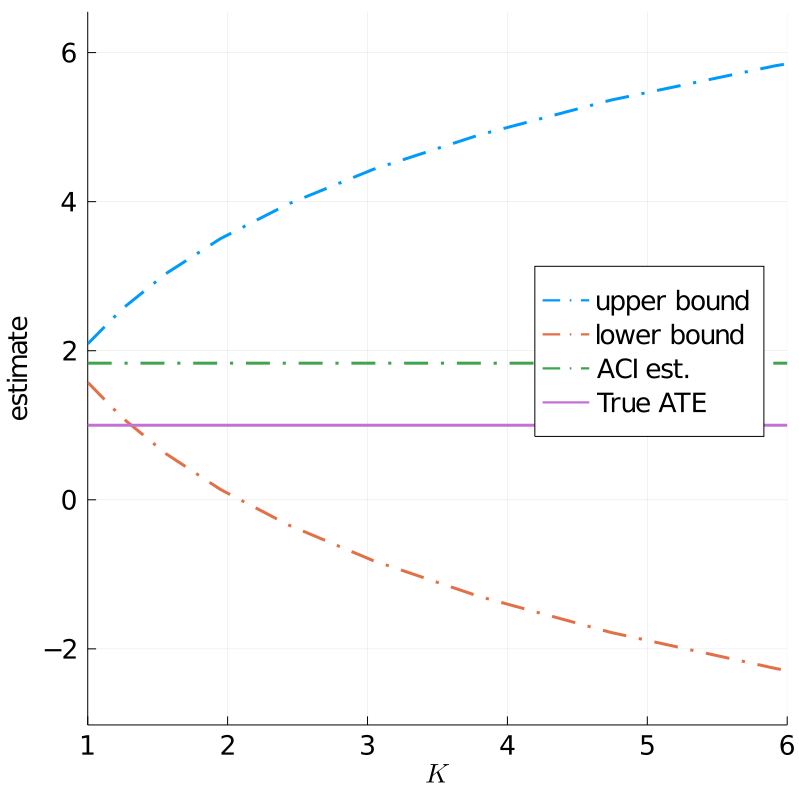
\includegraphics[width=0.6\textwidth]{../code/fig1.png}
        \caption{One realization}
        \label{fig:fig1}
    \end{figure}
\end{frame}

\begin{frame}{Simulation Results}
    \begin{figure}
        \centering
        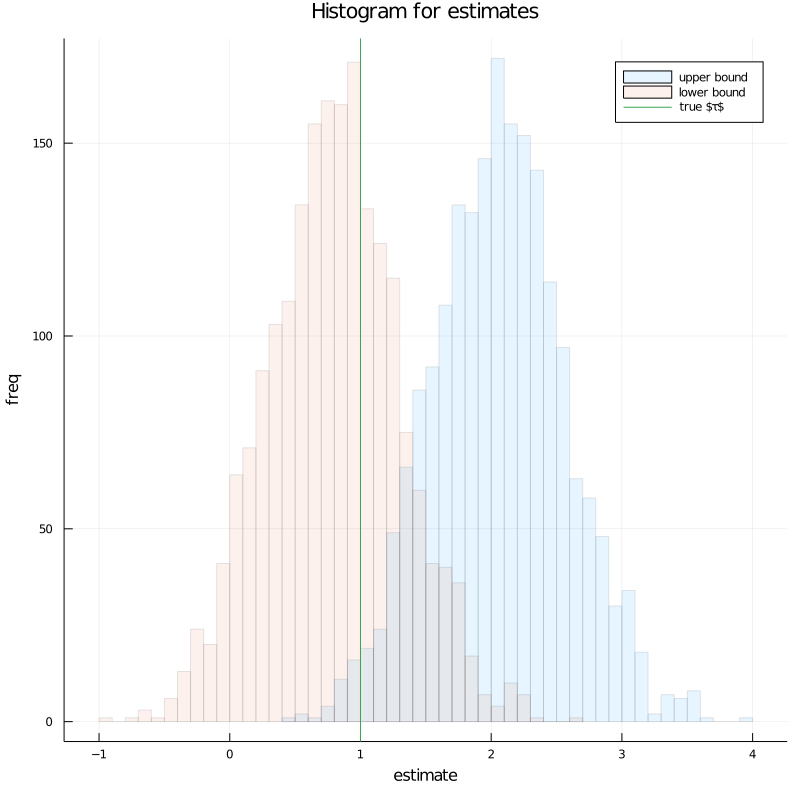
\includegraphics[width = 0.6 \textwidth]{../code/fig2.png}
        \caption{Histogram of Simulated Bounds}
        \label{fig:fig2}
    \end{figure}
\end{frame}

\begin{frame}
    \begin{table}
        \begin{adjustbox}{width=0.8\textwidth, totalheight=\textheight-2\baselineskip,keepaspectratio}
        \centering
    \begin{threeparttable}
    \caption{Monte Carlo Results: $B = 2000, \tau = 1, K = H = 1$}
        \begin{tabular}{| c | c | c | c | c |}
        \hline $\mathrm{n}$ & $\widehat{\tau}^{-}(\widehat{\tau}^{+})$ & \text {Std. dev. of } $\widehat{\tau}^{-}(\widehat{\tau}^{+})$ & \text {Coverage } \\
        \hline 500 & 1.038 & 0.732  & 0.9485 \\
        1000 & 1.039 & 0.495  & 0.9455 \\
        2000 & 1.029 & 0.357 & 0.947 \\
        \hline
        \end{tabular}
        \label{tab:tab1}
    \begin{tablenotes}
      \small
      \item Coverage statistics from $B = 2000$ simulations generated from the model specified above. The true ATE in the simulation is $\tau = 1$, and unobserved confounding is chosen such that simulation satisfies $K = H = 1.5$. Std. dev. of $\tau^-$ refers to standard deviation between simulation runs (likewise for $\tau^+$. Coverage is for estimated 95\% confidence intervals $(\hat{\tau}^- - 1.96 \hat{\sigma}^-, \hat{\tau}^+ + 1.96 \hat{\sigma}^+)$. In this case, $\tau^-$ and $\tau^+$ coincide. 
    \end{tablenotes}
  \end{threeparttable}
\end{adjustbox}
  \end{table}
\end{frame}


\begin{frame}

    \begin{table}
        \begin{adjustbox}{width=\textwidth, totalheight=\textheight-2\baselineskip,keepaspectratio}
        \centering
    \begin{threeparttable}
    \caption{Monte Carlo Results: $B = 2000, \tau = 1, K = H = 1.2$}
        \begin{tabular}{|c|c|c|c|c|c|}
        \hline $\mathrm{n}$ & $\widehat{\tau}^{-}$ & \text {Std. dev. of } $\widehat{\tau}^{-}$ & $\widehat{\tau}^{+}$ & \text {Std. dev. of } $\widehat{\tau}^{+}$ & \text {Coverage } \\
        \hline 500 & 0.803 & 0.710 & 2.080 & 0.716& 0.9895 \\
        1000 & 0.796 & 0.480 & 2.058 & 0.484 & 0.9945 \\
        2000 & 0.802 & 0.363 & 2.055 & 0.365 & 0.9950 \\
        \hline
        \end{tabular}
        \label{tab:tab2}
    \begin{tablenotes}
      \small
      \item Coverage statistics from $B = 2000$ simulations generated from the model specified above. The true ATE in the simulation is $\tau = 1$, and unobserved confounding is chosen such that simulation satisfies $K = H = 1.5$. Std. dev. of $\tau^-$ refers to standard deviation between simulation runs (likewise for $\tau^+$. Coverage is for estimated 95\% confidence intervals $(\hat{\tau}^- - 1.96 \hat{\sigma}^-, \hat{\tau}^+ + 1.96 \hat{\sigma}^+)$. These are conservative because the true model cannot simultaneously be upward biased and downward biased. Therefore, we would expect a model under worst-case confounding to converge to 97.5\% coverage.
    \end{tablenotes}
  \end{threeparttable}
\end{adjustbox} 
  \end{table}

\end{frame}

\section{Plans}

\begin{frame}{Plans}
    \begin{itemize}
        \item Wrap things up. check code, proof, etc... and rewrite the paper.
        \item Several remaining problems
        \item  Sharpness of the bounds
        \begin{itemize}
            \item Even when a single lower bound is sharp, the upper bound cannot be simultaneously sharp
            \item What if $U$ and $V$ are not independent? Correlation of the confounders
        \end{itemize}
        \item Which standard error, bootstrap or large sample approximation?
        \item Introducing covariates (Probably won't be able to finish)
        \item Continuous $S$ (Probably won't be able to finish)
    \end{itemize}
\end{frame}

\end{document}